%
% include the class file for USI-INF Technical Reports
%
\documentclass{usiinftr}
\usepackage{float}
\usepackage{amsmath}
\usepackage{slashbox}
\usepackage{subfigure}
\usepackage{listings}
\usepackage{algorithm}
\usepackage{algorithmicx}
\usepackage[noend]{algpseudocode}

%%%%%%%%%%%%%%%%%%%%%%%%%%%%%%%%%%%%%%%%%%%%%%%%%%%%%%%%%%%%%%%%%%%%
\newcommand{\der}{\operatorname{d\!}{}}
\begin{document}

\title{\bf Bayesian Additive Regression Tree (BART) \\ {\normalfont An overview of applications of Bayesian methods in regression }}
\author{Glejdis Shk\"embi}{\dagger}
\author{Franciskus Xaverius Erick}{\dagger}

\affiliation{\dagger}{Faculty of Engineering, Friedrich-Alexander Universit\"at Erlangen-N\"urnberg, Germany}

%
% by default, the current month and year are used as the publication date
% of your Technical Report; if you want to change this, then you can do it here, e.g.
%
%\date{February~\the\year}
%\date{August 2011}

\maketitle

\begin{abstract}
Classification and regression tree are some of the most relevant machine learning models used for a wide range of machine learning applications. In this paper, we discuss in detail the Bayesian Additive Regression Tree, which applies various concepts of Bayesian inference to perform Bayesian ensemble learning of multiple tree models with added regularization effects. We will first discuss the mathematical backgrounds of CART models, Bayesian inference methods such as Markov Chain Monte Carlo, Metropolis-Hastings algoirthm and Gibbs sampler. We explore in detail the ensembling of the trees, the prior tree regularization models and the specialized backfitting MCMC within Gibbs algorithm used to infer the posterior distributions. We will then test implementations of BART models in R and test them against diabetes dataset. Furthermore, the results will then be compared with results obtained from regression tree and random forest models. Lastly, the BART, classical regression tree and random forest models are tested on a synthetic dataset and their performance are then evaluated.
\end{abstract}

\section{Motivation}
Diabetes Mellitus is considered to be a global public health emergency. According to current worldwide estimates, this illness affects 415 million individuals and is expected to impact 642 million by 2040 \cite{27}. The most concerning part is that an addition of 193 million people with diabetes are undiagnosed \cite{27}. This is due to the often mild or asymptomatic character of the disease, particularly in type 2 diabetes. Consistently high blood glucose levels can lead to major life-changing and life-threatening consequences, such as hypertension, dyslipidemia, microalbuminuria and overt diabetic nephropathy \cite{27}. Diabetes kills 5 million individuals globally each year as a result of such complications, the majority of whom die prematurely. Being able to predict the progression of the disease at an early stage would facilitate the work of the medical workers and help in early correct treatment in order to prevent aggravation.  Therefore, in this paper we use a very powerful statistical model and try to analyse the data of 442 patients, including information such as age, sex, body-mass index (BMI), average blood pressure (BP), to predic the disease progression one year after the baseline. 
Bayesian Additive Regression Trees (BART) model recursively creates regression trees with variable hyperparameter distributions, including number of nodes, number of terminal nodes and depth of the tree \cite{16}. Since all parameters and hyperparameters are assumed to be non-parametric, the parameter distributions are recorded from recursive sampling from the Metropolis-Hastings algorithm \cite{16}. In contrast to the ensemble methods, in BART the Bayesian posterior distributions are computed in order to approximate the nonparametric model parameters. BART reduces the risk of overfitting by using regularization prior which limits the weights given to trees with small values \cite{16}. 

In this research paper, we aim to show the power of BART model through a real world application using the diabetes data which is free and publicly available on Hastie, Tibshirani,
Wainright website \cite{24}, and compare such a model with classical CART and Random Forests.  

\section{Mathematical Background}
In this section ,we will cover the notion of Classification and Regression Trees (CART), which gives a framework for the implementation of BART. 
Afterwards, we will introduce the main aspects of the Bayesian inference methods used in BART, namely Markov Chain Monte Carlo (MCMC), Metropolis-Hastings algorithm, and Gibbs sampler. The details in how these Bayesian inference methods are applied in the modelling of BART is also given afterwards. Furthemore, short theoretical background to random forest is also given.

\subsection{Classification and Regression Trees - CART}
The Classification and Regression Tree analysis, first introduced by Breiman et al. in 1984, is a well known decision tree method used in constructing predictor variables from the data. It builds a binary decision tree based on some splitting rule on the predictors \cite{1}. Regression trees are used for variables with continuous or ordered discrete values, while classification trees are intended for variables with a finite number of unordered values. Moreover, for regression trees, the prediction error is commonly assessed as the squared difference between the observed and predicted values, while for classification trees the prediction error is evaluated in terms of misclassification cost \cite{2}.

In a classification task, we have a training set with n observations, a class variable Y such that Y $\in {1, 2, \cdots, k}$ and the predictor variables $X_1, \cdots ,X_p$ with fixed dimensionality p and we try to find a model that better predicts the class Y given new values of X \cite{1}. The CART technique for classification problems produces rectangular sets $A_j$ by recursively partitioning the data set a single X variable at a time into disjoint sets $A_1,\cdots, A_j$ and fitting a single prediction model within each partition \cite{2}. The partitioning is repeated until a node is reached for which no split enhances homogeneity, at which point splitting is stopped and this node becomes a terminal node \cite{1}. This partitioning can be visually represented with a decision tree. In figure 1.0 we see a classification tree model with three classes labeled 1, 2 and 3, where the partitions are on the left and the decision tree is on the right. The root node of the tree represents the entire data set, and at each node, if the condition is satisfied, a case is assigned to the left child node. Moreover, the predicted class is beneath each leaf node \cite{2}. In contrast, in a regression task, the Y variable takes ordered values and we are trying to fit to each node a regression model to give predicted values of Y \cite{2}.

\begin{figure}[h!] 
\centering
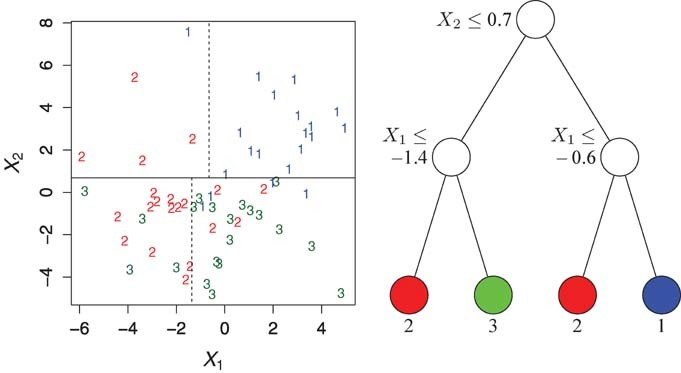
\includegraphics[width=0.7\textwidth]{images/image114.png}
\caption{Partitions (left) and decision tree structure (right) for a classification tree model with three classes labeled 1, 2, and 3 \cite{2}.}
\label{VarImp}
\end{figure}

The algorithm starts at the root node of the tree and grows itself as follows \cite{3}: 
\begin{itemize}
\item Step 1: Explore every possible split on each predictor variable. Binary questions are typically used to produce binary splits.
\item Step 2: Select and apply the best split (ie. selects the best feature which helps us better predicting the target class).
\item Step 3: Recursively proceed in this way until a stopping criterion is reached. 
\end{itemize}

The stopping criterion is reached when \cite{4}:
\begin{itemize}
\item The node's examples all belong to the same class.
\item There are no features remaining to distinguish between samples.
\item The tree has grown to the predetermined size limit. 
\item The first problem for a decision tree is determining which feature to split on.
\end{itemize}

Purity refers to the degree to which a subset of examples contains just a single class, and any subset made of only a single class is pure \cite{4}. There are several purity metrics that may be used to choose the optimal decision tree splitting candidate. C5.0 and CART are two algorithms for classification that follow this approach. They are both very similar, however, C5.0 uses entropy for its impurity measure, while CART uses the Gini index \cite{2}. Entropy is a measure of randomness or disorder within a set of class values. Mathematically, the entropy is formulated as follows: 

\begin{equation}
E(S)=\sum_{i=1}^{c}-p_{i} \log _{2} p_{i},
\end{equation}

where S represents the segment of data, c the number of different classes and p the probability of the values being part of class i \cite{4}. When entropy is equal to 0, this indicates that the set is completely homogeneous. The higher the entropy, the more diverse the set is, which means that less information is provided about other data points that may belong in the set. The goal of C5.0 is to find splits that reduce entropy,  hence enhancing homogeneity within the groups \cite{4}. Now, using entropy, the Information Gain of a feature F can be calculated as shown below\cite{4}:

\begin{equation}
\text{InfoGain(F) = Entropy(S1) - Entropy(S2).}
\end{equation}

The higher the information gain is, the more homogeneous the set created after the split on this feature is. On the other hand, Gini index calculates the "impurity" of a feature with respect to the classes \cite{5}. More specifically, it indicates the probability of a specific feature to be classified incorrectly when we do random selection. It is given by the following formula \cite{5}:

\begin{equation}
\sum \sum_{j \neq i} p_{i} p_{j}=\left(\sum p_{i}\right)^{2}-\sum p_{i}^{2}=1-\sum p_{i}^{2}
\end{equation}

Breiman et al. (1984) points out that the stopping rules in Step 3 do not work very well in practical applications, as the tree tends to become too large and has too few data points in each terminal node, making its decisions overly specific and increasing the risk of model overfitting. Therefore, to address this issue, there is the need to prune the tree. Pruning a decision tree is the process of reducing its size in order to generalize better to unseen data \cite{4}. There are two types of decision tree pruning: pre-pruning or post-pruning. In pre-pruning, also known as early stopping, we let the tree grow until it reaches a predefined number of decisions or until there is only a small number of examples in the node, and then we stop it \cite{4}. In this way we avoid doing extra work, however, it is difficult to know whether this way we leave out subtle but important patterns. On the other hand, in post-pruning, we intentionally allow a very large tree to grow and then we use pruning criteria to reduce its size to a more appropriate level \cite{4}. This type of pruning ensures us that all of the important information is discovered. 
	
Some of the main advantages of the decision trees include \cite{4}:
\begin{enumerate}
\item Are easy to be interpreted even by non-statisticians;
\item Work well with missing variables;
\item Are invariant under transformations in the predictor space;
\item There are extensions: Bayesian version of CART.
\end{enumerate}

Moreover, some of the drawbacks are:
\begin{enumerate}
\item A lot of data is needed as the tree-space is big;
\item Might not result in the "best" model;
\item There is selection bias for the splits;
\item May lead to overfitting.
\end{enumerate}

\subsection{Markov Chain Monte Carlo - MCMC}
In Bayesian statistics, one would normally propose a prior distribution of the samples and these priors are updated according to the likelihood of observations from the samples. In this way, the posterior distribution, which describes the the distribution of the samples given the obtained likelihood, can be determined. The main formula of this update process is given as follows \cite{21}.

\begin{equation} \label{Bayes}
p(\theta \mid y) = \frac{p(\theta)p(y \mid \theta)}{p(y)} = \frac{p(\theta)p(y \mid \theta)}{\int p(\theta)p(y \mid \theta) d\theta}
\end{equation}

The integral in the denominator which represents the marginal likelihood of y can be treated as a normalizing constant of the whole expression. For very simple distributions, this normalizing constant can be determined analytically. However, in real life situations, the likelihoods obtained can get highly complex in expression,which makes it impossible to evaluate this integral term. There are various methods that can be used instead to approximate the posterior distribution, without the need to evaluate such complicated integrals. One of the most common method is Markov Chain Monte Carlo, or MCMC.

Markov Chain Monte Carlo, first introduced by physicists at Los Alamos in the 1940's, is a computer-based sampling approach, which, by randomly sampling values out of the distribution, allows one to describe a distribution without knowing in advance all of its mathematical properties \cite{20}. As written in the name, MCMC combines two properties: Monte Carlo and Markov Chain. 

Monte Carlo estimates the properties of a distribution by exploring random samples from the distribution, while Markov Chain generates random samples sequentially where each random sample is used as a building block to generate the next random sample \cite{20}. In other words, rather than computing the mean of a normal distribution from its equations, in Monte Carlo approach we draw a large number of random samples from this normal distribution and then compute the sample mean, which is much easier than computing the mean directly from the normal distribution's equations.

Markov Chain is a sequence $X_1,X_2, X_3, \cdots$ of random variables if the conditional distribution of $X{n+1}$ given $X_1,X_2, X_3, \cdots, X_n$ depends only on $X_n$ \cite{21}.That is to say that the future is independent of the past given the present \cite{21}. This is known under the name of Markov Property. In MCMC, the state of the Markov chain $\theta^{t}$ is a drawn sample that corresponds to a certain distribution at iteration step $t$. Due to the Markovian property, the states at current iteration only depends on the states of the previous iteration step. The goal of MCMC is to simulate the posterior distribution $p(\theta \mid y)$, which can be treated as the target distribution, by iteratively constructing Markov Chain which stationary distribution converges to the target posterior distribution. 


\subsection{Metropolis-Hastings algorithm}
Computationally, the generation of Markov chains in MCMC can be realized through Metropolis-Hastings algorithm. Metropolis-Hastings algorithm employs proposal distribution $q(\theta^{t},\theta^{t-1})$, from which each state $\theta^{t}$ at iteration step $t$ is proposed, eventually leading to the desired Markov chain. The proposed state depends on the state from the previous iteration $\theta^{t+1}$. With Metropolis-Hastings algorithm, one would be able to approximate any probability density function $\pi(x)$ using only a proposal distribution function $q(x)$ and a function $f(x)$ which is proportional to the real probability density function $\pi(x)$ \cite{28}.  This is especially useful in the context of approximating posterior distribution function as of \ref{Bayes}. Since the posterior distribution is proportional to the numerator of the right hand side of the equation, one would only need to evaluate the numerator and propose a proposal distribution to approximate the posterior distribution by Metropolis-Hastings algorithm, without the need to analytically compute the complex integral in the denominiator.

In general, the symmetric Metropolis-Hastings ( $q(x_t,x_{t-1}) = q(x_{t-1},x_t)$ ) algorithm with proposal distribution function $q(x)$ and function $f(x)$ can be described in the following pseudocode \cite{21}.

\begin{algorithm}
  \caption{General Metropolis-Hastings algorithm} \label{algMH}
  \begin{algorithmic}[1]
    \Statex
    \Function{MH}{$x_0, n$}
    \State {$x_1 = x_0$}
    \For { $i \gets 2 \textrm{ to }  n $ }
    	\State { $ y \gets q(x_i,x_{i-1})$ }
    	\State { $ \alpha \gets \textrm{min}(1, f(y)/f(x_{i-1}))$ }
    	\State { $ u \gets \textrm{runif}(1) $}
    	\If { $ \alpha \geq u $ }
    		\State{ $ x_i = y$}
        \Else
            \State{ $ x_i = x_{i-1}$}
        \EndIf
    \EndFor
    \State \Return{$x$}
    \EndFunction
  \end{algorithmic}
\end{algorithm}

In the pseudocode, the first state is initialized with a given initial state. The candidate next state is then proposed from the proposal distribution given the previous state. The acceptance ratio $\alpha$ evaluate the probability of moving from the current state to the candidate state. If this acceptance ratio value is lower than a randomly generated number from a uniform distribution ranging from 0 to 1, then the candidate state is taken as the next state. Otherwise, the next state would simply just be the current state ( no move from the current state ). This is iterated until a maximum number of iteration $n$ is reached. In the case when the proposal distribution is not symmetric, the acceptance ratio would be $ \alpha \gets \textrm{min}\left(1, \frac{f(y)q(y,x_{i-1})}{f(x_{i-1})q(x_{i-1},y}\right)$ instead. 

Since the proposal distribution depends on the previous state, this very algorithm is also a case of random walk Metropolis Hasting \cite{21}. The Metropolis-Hasting algorithm is relatively easy to implement and does not suffer from curse of dimensionality, which is a well known issue for importance and rejection sampling. Therefore, the Metropolis-Hastings is currently very widely used for Bayesian inference. 

A convergence to the target distribution is also guaranteed. However, care needs to be taken of with regards to the proposal distribution used. If the variance of the proposal distribution is too low, the states proposed would be too close and similar to each other, resulting to a higher degree of autocorrelation and subsequently a slow convergence. If the variance of the proposal is too high, there would also be a higher amount of rejected candidates, which in turn result to slow convergence \cite{30}. To ensure that the final distribution is indeed approximate to the target distribution, a burn-in period is also taken into consideration \cite{29}. This means that the proposed states from the first $n$ ( typically 1000 iterations ) are ignored as the initial distributions may not reflect the true converged target distribution.


\subsection{Gibbs Sampler} 
Gibbs sampling can be considered to be a special case of Metropolis-Hastings algorithm, whereby the acceptance rate is always taken as 1 \cite{21}. It is specially used when sampling multivariate distributions, whereby a "correct" proposal distribution function that ensures reasonable convergence speed may not be easily determined. For Gibbs sampling, the update of each dimension of the state $\theta^{t}_d$ is given as the conditional distributions of each dimension for the dimensions $d = 1,2,\cdots,D$. In general, Gibbs sampling algorithm is done in the following pseudo-code \cite{21}:

\begin{algorithm}[h]
  \caption{General Gibbs sampler algorithm} \label{algGibbs}
  \begin{algorithmic}[1]
    \Require{The initial state of $\theta$ has already been initialized,$ \theta^{1} \neq \textrm{NULL}$}
    \Statex
    \Function{Gibbs}{$\theta, n$}
    \For { $i \gets 2 \textrm{ to }  n $ }
    	\State { $ \theta_1^{i} \gets \pi( \theta^{i}_1 \mid \theta^{i-1}_{2},\theta^{i-1}_{3}, \theta^{i-1}_{4}, \cdots, \theta^{i-1}_{D} )$ }
    	\State { $ \theta_2^{i} \gets \pi( \theta^{i}_2 \mid \theta^{i}_{1},\theta^{i-1}_{3},\theta^{i-1}_{4}, \cdots, \theta^{i-1}_{D} )$ }
    	\State { $ \theta_3^{i} \gets \pi( \theta^{i}_3 \mid \theta^{i}_{1},\theta^{i}_{2},\theta^{i-1}_{4}, \cdots, \theta^{i-1}_{D} )$ }
    	\State { $ \vdots $ }
    	\State { $ \theta_D^{i} \gets \pi( \theta^{i}_D \mid \theta^{i}_{1},\theta^{i}_{2},\theta^{i}_{4}, \cdots, \theta^{i}_{D-1} )$ }
    \EndFor
    \State \Return{$\theta$}
    \EndFunction
  \end{algorithmic}
\end{algorithm}

Thus for Gibbs sampler, one would only required the conditional distributions in order to approximate the 
target distribution. As the acceptance rate is always 1, no additional proposal distribution matching is required \cite{21}. However, this method can only be done when the conditional distributions can be sampled from. This is always not the case as for some distributions, the conditional distribution expressions can even be hard to obtain \cite{21}. Furthermore, the acceptance rate of 1 also comes with the cost of the inability to adapt to the cases when the states are highly correlated ( high autocorrelation ). This would also lead to a slower convergence as the high correlation would makes it harder for the algorithm to cover the whole target distribution \cite{21}. As in the classic Metropolis-Hastings algorithm, burn-periods need to be taken into account to ensure convergence of the Markov Chain.

\subsection{Bayesian Additive Regression Tree}
As previously mentioned, the classical CART is prone to overfitting. This leads to various research into a more Bayesian approach to the decision trees. By applying Bayesian framework, the data can overcome the assumptions about the depth of trees and the shrinkage needed. The Bayesian framework encodes what is typically an algorithmic approach in a likelihood framework to generate coherent uncertainty intervals.

 Chipman et al. (2010 )\cite{7} proposed a Bayesian "sum-of-trees" model, which is defined by a prior and a likelihood, where each tree is constrained by a regularization prior in order to be a weak learner.  Fitting is achieved by a specialized iterative backfitting MCMC algorithm. This "sum-of-trees" model results to be adaptive and very flexible, where each individual tree describes a different part of the underlying mean function \cite{7}. The "sum-of-trees" model differ from other ensemble methods that fit a linear combination of trees, such as boosting \cite{11}, random forests \cite{10}, bagging \cite{12}. In bagging and random forest models we do random sampling and stochastic search to create a collection of independent trees, and then combine their results by averaging. It is worth noticing that from various literatures, BART performs better compared to LASSO \cite{8}, gradient boosting \cite{9}, random forests \cite{10} and neural networks with one hidden layer. 
 
\subsubsection{Sum of Trees Model}
Chipman et al. (2010) consider the problem in which a dependent variable Y needs to be predicted using the p dimensional input vector $\textbf{x} = (x_1,\cdots, x_p)$ \cite{7}:

\begin{equation}
Y=f(x)+\epsilon, \quad \epsilon \sim N\left(0, \sigma^{2}\right),
\end{equation}

where function f(x) is unknown. Bayesian statistics aims to approximate the mean of Y given x by the sum of m trees. Each tree is represented by the $g_j$ function \cite{7}:

\begin{equation} \label{sum}
f(x)=E(Y \mid x) \approx h(x) \equiv \sum_{j=1}^{m} g_{j}(x)
\end{equation}

We further break down the components of the trees in the $g_j$ function. We define $T_j$ to be the j-th tree with the corresponding terminal nodes $M_j = \{ \mu{ij}, \cdots, \mu{bj} \}$. b defines the amount of terminal nodes of the corresponding tree. Thus, equation \ref{sum} can be rewritten as follows \cite{7}.

\begin{equation} \label{sum1}
f(x)= \sum_{j=1}^{m} g(x;T_j,M_j)
\end{equation}

\begin{figure}[h!] 
\centering
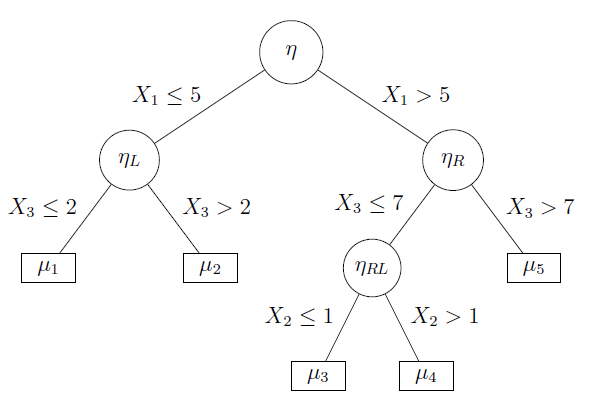
\includegraphics[width=0.6\textwidth]{images/image113.png}
\caption{A binary tree example.}
\label{bintree}
\end{figure}

\subsubsection{Regularization Priors}\label{prior}
Bayesian priors are the main features in BART which enforce regularization to the added regression trees, thus ensuring that the trees do not get too significantly big, adapt to the data well while at the same time reduce overfitting \cite{7}. The prior specifications, stated in Chipman et al. (2010) \cite{7}, will be described in more detail here.

There are three priors used for regularization, namely \cite{7}:
\begin{enumerate}
\item $\pi(T_j)$ the prior of the tree structure itself,
\item $\pi(M_j \mid T_j)$ the prior of the leaf structures given the tree structure, 
\item $p(\sigma^2)$ the residual variance.
\end{enumerate}

Each of the prior are discussed in more details as follows.
\begin{enumerate}
\item $\pi(T_j)$ the prior of the tree structure itself. This prior itself has 3 separate components
			\begin{enumerate}
				\item The probability that the node depth $d = 1,2,\cdots,n$ is not terminal. The node depth is defined as the distance from the root node. This is expressed as 
			\begin{equation}\frac{\alpha}{(1+d)^{\beta}}, \quad \alpha \in (0,1), \beta \geq 0 . \end{equation}
			Where $\alpha$ and $\beta$ are hyperparameters to be tuned. This component enforces regularization on the depth of the trees itself so that they do not get too large. Chipman et al. (2010) recommends default values of $\alpha = 0.95$ and $\beta =2$ \cite{7}.
				\item The probability that the i-th feature out of p features of data is taken to be the decisive splitting variable for a node. Chipman et al. (2010) \cite{7} uses uniform distribution over all the possible features p.
				\item The probability that for the selected i-th feature , that a certain value of cut off point is used. Chipman et al. (2010) \cite{7} uses uniform distribution over all the discrete possible splitting values of that certain feature.
			\end{enumerate} 
\item The prior $\pi(M_j \mid T_j)$ can be expressed as the product of all probabilities of the observed terminal nodes given the tree.
\begin{equation}\pi(M_j \mid T_j) = \prod_i p(\mu_{ij} \mid T_j). \end{equation}

Chipman et al. (2010) \cite{7} recommends a normal distribution for the prior $p( \mu_{ij} \mid T_j) \sim \mathcal{N}(0, \sigma^2_{ \mu })$, whereby $ \sigma_{ \mu } = \frac{0.5}{k \sqrt{m}}$  and k is a hyperparameter to be tuned. The default value of k is taken as k = 2. Thus, this term would ensure that the leaves output get closer to 0 ( the center of the normal distribution ) when the variance term $\sigma_{ \mu}$ gets smaller.
\item $p(\sigma^2)$, which is the residual variance. The residual variance helps to impose regularization effect on the whole term such that the model will not overfit to the training data. This prior is modelled with the conjugate prior inverse chi square distribution, which is none other than a special case of inverse Gamma distribution, as follows \cite{7}.
\begin{equation}p(\sigma^2) \sim \frac{\nu \lambda}{\chi_{\nu}^2}. \end{equation}

With $\lambda$ and $\nu$ as the hyperparameters. More frequently, another hyperparameter is $q$ is chosen in order to determine the hyperparameter $\lambda$ from looking at the prior distribution. While there are more detailed approaches to choosing the hyperparameters, for convenience, Chipman et al. (2010) \cite{7} additionally suggests to use the default values of $\nu = 3$ and $q = 0.90$ to avoid overfitting and yield good results.
\end{enumerate}

Taking these prior components into account, the resulting regularization prior distribution is none other 
than \cite{7}:

\begin{equation}
\begin{aligned}
p\left(\left(T_{1}, M_{1}\right), \ldots,\left(T_{m}, M_{m}\right), \sigma\right) &=\left[\prod_{j} p\left(T_{j}, M_{j}\right)\right] p(\sigma) \\
&=\left[\prod_{j} p\left(M_{j} \mid T_{j}\right) p\left(T_{j}\right)\right] p(\sigma)
&= \left[\prod_{j}  \prod_{i} p\left(\mu_{i j} \mid T_{j}\right) p\left(T_{j}\right)\right] p(\sigma)
\end{aligned}
\end{equation}

The likelihood is taken to be the likelihood of outputting certain values of Y given the tree models with its specifications. This likelihood is modelled with a normal distribution, with the mean being the best guess possible for the specific configurations of the added regression trees \cite{7}.

\begin{equation}
y_l \sim \mathcal{N}(\mu_l, \sigma^2)
\end{equation}



\subsubsection{Posterior distributions}
With the priors and likelihood specified in the previous sections, the posterior distribution is now left to be approximated. Direct analytical evaluation of the posterior distribution is not possible as it is not feasible to analytically compute the marginal likelihood from the non-trivial prior distribution functions. Chipman et al. (2010) \cite{7} proposed a specialized backfitting MCMC algorithm to approximate the posterior distribution. The specialized backfitting MCMC algorithm was developed off a similar backfitting MCMC algorithm proposed by Tibshirani et al. (2000) \cite{31} for approximating posterior distributions of generalized additive models. The pseudo-code for the specialized backfitting MCMC algorithm algorithm basing on the version summarized by Lakshminarayanan et al. (2015) is as follows \cite{32}.

\begin{algorithm}[h]
  \caption{Specialized backfitting MCMC algorithm} \label{algSpc}
  \begin{algorithmic}[1]
    \Statex
    \Function{SpecialbackfitMCMC}{$X,Y,$ various BART hyperparameters}
    \For { $j \gets 1 \textrm{ to }  m $ }
    	\State { $ T_j^{(0)} \gets $ single node initialization }
    	\State { Sample $ M_j^{(0)} \mid T_j^{(0)} $ }
    \EndFor
    \For { $i \gets 1 \textrm{ to }$ maxiter }
    	\State { Sample $\sigma^(i) \mid (T_1^{(i-1)},M_1^{(i-1)}),(T_2^{(i-1)},M_2^{(i-1)}), \cdots, (T_m^{(i-1)},M_m^{(i-1)}), \boldsymbol{\varepsilon}  $ }
    	\For { $j \gets 1 \textrm{ to }  m $ }
    	    \State { Compute Residual $R_{-j}^i$ }
    		\State { Sample $ T_j^{(i)} \mid R_{-j}^i, \sigma^2 $ }
    		\State { Sample $ M_j^{(i)} \mid T_j^{(i)}, R_{-j}^i, \sigma^2 $ }
    	\EndFor
    \EndFor
    \EndFunction
  \end{algorithmic}
\end{algorithm}

The specialized backfitting MCMC algorithm is fundamentally based on Gibbs sampling algorithm. The first Gibbs iteration is done as initialization of the tree and leaves parameters for the subsequent Gibbs sampling iterations. Note the residual term $R_{-j}$ fitted to all trees except for the tree to be sampled from. The residual term is given by the following expression \cite{7}.

\begin{equation}
\boldsymbol{R}_{-j}:=\boldsymbol{y}-\sum_{t \neq j} \mathcal{T}_{t}^{\mathcal{M}}(\boldsymbol{X})
\end{equation}

There are three main conditionals that are sampled within each Gibbs iteration.

\begin{enumerate}
\item $ T_j^{(i)} \mid R_{-j}^i, \sigma^2 $. This is the conditional of the tree structure conditioned on the special residual term from the remaining trees and the residual variance. This component is sampled by an additional Metropolis-within-Gibbs sampler that decides one of the four possible steps ( GROW, PRUNE, CHANGE, SWAP ) to be taken against the j-th tree structure of the current Gibbs iteration. For each of the decision, the acceptance ratio of each move decision is evaluated similarly to how acceptance ratios are calculated in the classic Metropolic-Hastings algorithm.
\item $ M_j^{(i)} \mid T_j^{(i)}, R_{-j}^i, \sigma^2 $ \cite{7}. This is the conditional of the leaves parameters conditioned on the j-th tree structure of the current Gibbs iteration, special residual term from the remaining trees and the residual variance. Since the prior and likelihood are both of normal distributions, the conditional can be directly sampled from a conjugate normal distribution with parameters calculated from the parameters of the priors and the likelihood.
\item $\sigma^(i) \mid (T_1^{(i-1)},M_1^{(i-1)}),(T_2^{(i-1)},M_2^{(i-1)}), \cdots, (T_m^{(i-1)},M_m^{(i-1)}), \boldsymbol{\varepsilon}  $. This is the conditional of the residual variance conditioned on all the tree structures, the corresponding leaves parameters and the whole residual term. The whole residual term for the entire tree structures can be calculated as follows \cite{7}.

\begin{equation}
\boldsymbol{\varepsilon}:=\boldsymbol{y}-\sum_{t=1}^m \mathcal{T}_{t}^{\mathcal{M}}(\boldsymbol{X})
\end{equation}
Since the prior is taken as the conjugate prior inverse chi-squared distribution, sampling from the posterior can be directly done from a conjugate inverse chi-squared distribution \cite{7}.
\end{enumerate}

\subsubsection{Recommended Hyperparameters}\label{rec}
In summary, the recommended hyperparameters for the modelling of the priors are  $\alpha = 0.95, \beta =2, \nu = 3, q = 0.90, \text{and} k = 2$. The recommended number of trees is taken as m = 200 \cite{7}. To ensure that the MCMC converges, a sufficient number of burn-in iterations needs to be taken into account.


\subsection{Random Forest}
Random forest, championed by Leo Breiman and Adele Cutler, is an ensemble method combining decision trees and bagging \cite{22}. Using the concepts of random feature selection and bagging, first, it generates a collection of trees, and then each of the trees votes for the most popular class \cite{4} (see Figure \ref{RF_fig}). To improve stability and accuracy of the regression models, bagging is being used. Bagging does random sampling with replacement. That is to say that  many different "copies" of the training data are created, then weak classifiers are applied to these "copies", and their result is combined. This will result in reduced variance and low overfitting \cite{23}. 


	Building the ensembles, for the k-th decision tree, a random vector k with identical distribution for all the trees in the forest is generated \cite{22}. These vectors are independent of all the previous random vectors $i$ where $i = 1,\cdots,k-1$. Next a tree is grown using the training set and the generated random vector \cite{22}. This results in a classifier $h(x,k)$ where $x$ denotes the input vector and $k$ denotes the generated random vector \cite{22}. Moreover, the trees are allowed to grow without pruning, which results in low bias.  Some of the main advantages of RF include\cite{4}:

\begin{itemize}
\item Can work with categorical and continuous features;
\item Can handle missing and noisy data;
\item Can perform well even with a large number of features as it selects only a subset of them. 
\end{itemize} 

\begin{figure}[h!] 
\centering
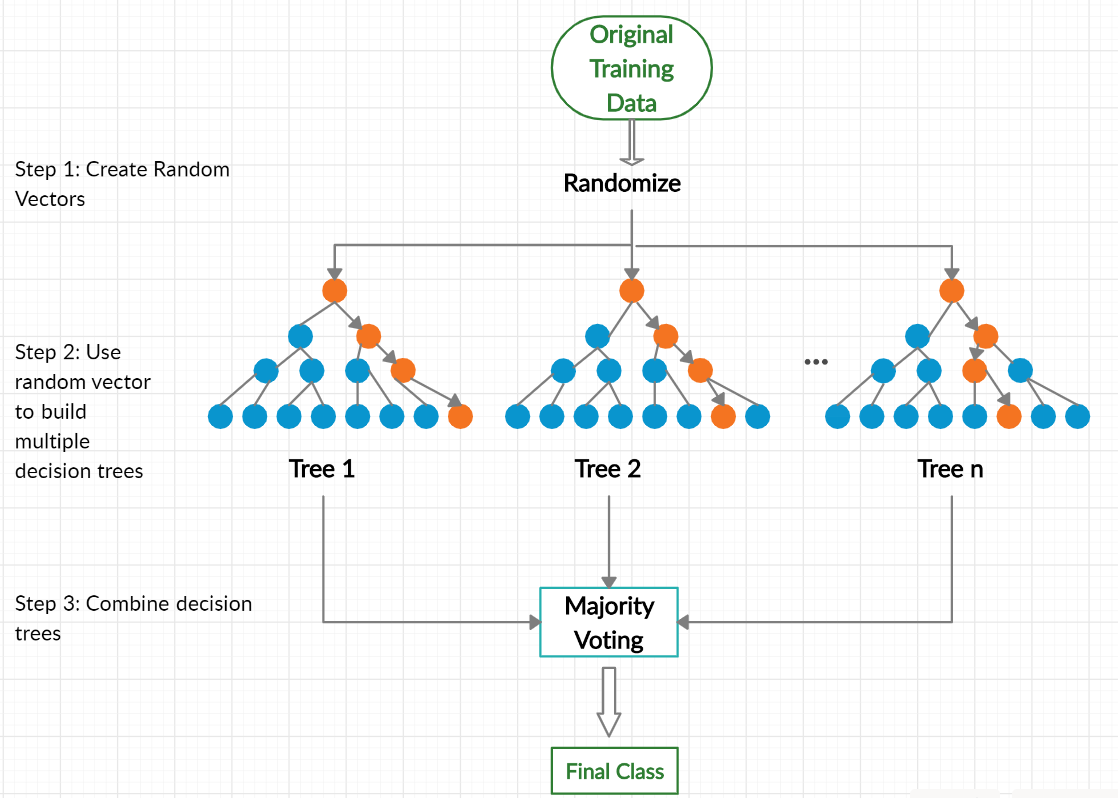
\includegraphics[width=0.7\textwidth]{images/image122.png}
\caption{Visual representation of the Random Forest Algorithm.}
\label{RF_fig}
\end{figure}

\section{Experiment Methods}
The experiments will be done in three parts parts. First experiment is to run a BART model in R and evaluate the results and its performance. This is done by utilizing a prewritten BART library in R called "bartMachine". The second part of the experiment is to compare the performance of the BART model itself with another BART model from another R library called "BART", a classic regression tree model, and a random forest model. In the third part, we will compare the performance of BART against the classic regression tree and random forest model trained on a synthetic dataset.

\subsection{Dataset}\label{dataset}
In this study, the diabetes data which is free and publicly available on Hastie, Tibshirani,
Wainright website, is being used \cite{24}. The dataset contains observations on 442 patients. The response of interest y is a quantitative measure of disease progression one year after baseline. The 442 diabetes patients were measured on 10 baseline variables:  age, sex, body-mass index, average blood pressure, and six blood serum measurements \cite{24}. Moreover, before the data is being used, they are first standardized to have zero mean and unit L2-norm \cite{24}. The complete data used in our experiments contains 64 feature variables. The first column is the response y, the next 10 columns are the age, sex, BMI, BP and the serum measurements, and the rest of the columns are the squares and products of the original 10. The statistical feature extraction is already performed in our dataset, therefore no further preprocessing is applied to the diabetes dataset. For all the tests, 75\% of the data is taken as the training data with the remaining 25\% as the test data.

\begin{table}[h!]
\centering
\caption{Original diabetes data \cite{25}}
\begin{tabular}{cccccccccccc}
\hline & AGE & SEX & BMI & BP & \multicolumn{5}{c} { Serum measurements } & Response \\
Patient & $\mathrm{x}_{1}$ & $\mathrm{x}_{2}$ & $\mathrm{x}_{3}$ & $\mathrm{x}_{4}$ & $\mathrm{x}_{5}$ & $\mathrm{x}_{6}$ & $\mathrm{x}_{7}$ & $\mathrm{x}_{8}$ & $\mathrm{x}_{9}$ & $\mathrm{x}_{10}$ & $\mathrm{y}$ \\
\hline 1 & 59 & 2 & $32.1$ & 101 & 157 & $93.2$ & 38 & 4 & $4.9$ & 87 & 151 \\
2 & 48 & 1 & $21.6$ & 87 & 183 & $103.2$ & 70 & 3 & $3.9$ & 69 & 75 \\
3 & 72 & 2 & $30.5$ & 93 & 156 & $93.6$ & 41 & 4 & $4.7$ & 85 & 141 \\
4 & 24 & 1 & $25.3$ & 84 & 198 & $131.4$ & 40 & 5 & $4.9$ & 89 & 206 \\
5 & 50 & 1 & $23.0$ & 101 & 192 & $125.4$ & 52 & 4 & $4.3$ & 80 & 135 \\
6 & 23 & 1 & $22.6$ & 89 & 139 & $64.8$ & 61 & 2 & $4.2$ & 68 & 97 \\
$\vdots$ & $\vdots$ & $\vdots$ & $\vdots$ & $\vdots$ & $\vdots$ & $\vdots$ & $\vdots$ & $\vdots$ & $\vdots$ & $\vdots$ & $\vdots$ \\
441 & 36 & 1 & $30.0$ & 95 & 201 & $125.2$ & 42 & 5 & $5.1$ & 85 & 220 \\
442 & 36 & 1 & $19.6$ & 71 & 250 & $133.2$ & 97 & 3 & $4.6$ & 92 & 57 \\
\hline
\end{tabular}
\end{table}


In the third part of the experiment, a synthetic dataset would be used to test the performance of the models in a controlled setting. A common synthetic dataset used for regression models is the Friedman dataset, first used in the publication of Multivariate Adaptive Regression Splines (MARS) \cite{33}. This dataset consists of covariates of x, whereby each covariate data consists of random numbers between 0 and 1 sampled from uniform distribution. The response y is determined from the following equation \cite{33}\cite{34}.

\begin{equation}\label{friedman}
\boldsymbol{y}=10 \sin \left(\pi \boldsymbol{x}_{1} \boldsymbol{x}_{2}\right)+20\left(\boldsymbol{x}_{3}-.5\right)^{2}+10 \boldsymbol{x}_{4}+5 \boldsymbol{x}_{5}+\mathcal{E}, \quad \mathcal{E} \sim \mathcal{N}_{n}\left(\mathbf{0}, \sigma^{2} \boldsymbol{I}\right)
\end{equation}

As from the equation, we can see that the response y only depends on 5 covariates. There are non-linear dependencies for the covariates $\boldsymbol{x}_{1}, \boldsymbol{x}_{2}, \text{
and} \boldsymbol{x}_{3}$ and linear dependencies for covariates $\boldsymbol{x}_{4} \text{
and} \boldsymbol{x}_{5}$. Therefore, using the Friedman data, we can test the performance of the models for non-linear, multivariate data in a controlled setting, whereby the exact dependencies of the covariates is known. This is in contrast with real datasets, whereby the exact dependencies and relationships between the covariates are not exactly understood. For our comparisons with Friedman dataset, we used the Friedman dataset function as implemented by Kappelner and Bleich \cite{14}. We use a generated Friedman dataset with 100 covariates, whereby only the first 5 covariates contribute to the output response as seen in equation \ref{friedman}. We use 500 training observations to train the models. The trained models are then tested on 500 test observations.

\subsection{Evaluation Metrics}
In our regression setting, to measure the performance of our models, R squared and root mean squared error (RMSE) are used. R squared is the proportion of variance explained by the model: 

\begin{equation}
R^{2}=1-\frac{\sum_{i=1}^{n}\left(y_{i}-\tilde{y}\right)^{2}}{\sum_{i=1}^{n}\left(y_{i}-\bar{y}\right)^{2}}
\end{equation}

The RMSE, which is the square root of the variance of the residuals, is given by the formula: 

\begin{equation}
R M S E=\sqrt{\frac{1}{n} \sum_{i=1}^{n}\left(y_{i}-\hat{y}\right)^{2}}
\end{equation}

It indicates how close the observed data points are to the model's predicted values. Lower values or RMSE indicate better fit, as RMSE measures how accurately our model predicts the response y.  

\subsection{BART R Libraries}
There are currently multiple implemented BART libraries in R. The "bayesTree" library was developed by Chipman et al. (2010) \cite{7}, sticking to the original implementation as specified in the literature. However, the "bayesTree" library does not support parallelization and detailed model diagnostics. In 2013, Kapelner and Bleich published their implementation of BART in their "bartMachine" library \cite{14}. The "bartMachine" library allows one to easily model a BART model, evaluate in detail statistics of the model fitting against datasets, use multiple computing cores, optimize the hyperparameters used for prior modelling, evaluate convergence of the MCMC and many other statistical tests. This allows us to evaluate the performance and statistics of our BART model in a very detailed manner. Another more recent BART library is "BART", developed by McCulloh and Sparapani in 2017 \cite{18}. This "BART" library provides various statistical testings and has higher compability with other libraries in R, which makes it easier for one to implement functionalities and tests for the created BART model. However, this "BART" library only supports multi-threading if MPI is installed in the user's computer. In addition, the "BART" library is still relatively in development and the features and functionalities of this library are still updated frequently up to this day. For this reason, we will use "bartMachine" as the main R library used to model and evaluate our BART model. The BART model implemented in "BART" library will be used solely for comparison. Aside from the functionalities and statistical tests available, each BART libraries also differ slightly in their implementation and interpretation of some prior parameters. As such, it is also worth investigating to see if the default implementations of BART in "bartMachine" and "BART" would return similar performance when trained with the same dataset. The following table summarize the features and differences of each of the three libraries as summarized by Sparapani in a BART Bootcamp lecture slide \cite{18}.

\begin{table}[h!]
\centering
\caption{Comparison of the different BART libraries in R \cite{18}.}
\begin{tabular}{l|lll} 
& BayesTree & BART & bartMachine \\
\hline Author(s) & Chipman & McCulloch & Kapelner \\
& McCulloch & Sparapani & Bleich \\
Computer language & $\mathrm{C}++$ & $\mathrm{C}++$ & java \\
Dependencies & None & Rcpp & rJava \\
Multi-threaded & No & Yes & Yes \\
predict function & No & Yes & Yes \\
Missing data handling & No & No & Yes \\
Variable selection & No & No & Yes \\
Variable importance & Yes & Yes & Yes \\
Tree transition proposals & 3 & 3 & 3 \\
Partial dependence plots & Yes & No & Yes \\
Continuous \& binary & Yes & Yes & Yes \\
Convergence diagnostics & Continuous & All & Continuous \\
Cross-validation & No & No & Yes \\
\hline
\end{tabular}
\end{table}




\section{Results and Discussion}
\subsection{First experiment results : bartMachine}
After the dataset is split according to 3:1 train:test ratio as specified in \ref{dataset}, the model is constructed with the default bartMachine model constructor. The default values of prior hyperparameters used in bartMachinde models are equal to the values specified in \ref{rec}, with the exception of number of trees which is taken as m = 50 instead of m = 200. As of the official documentation of bartMachine \cite{12}, the burn-in Gibbs iterations are 250 and the default post burn-in Gibbs iterations are 1000. 

\subsubsection{Results}
By using the default parameters, we obtain an in-sample RSME value of 41.6 and in-sample R-squared value of 0.708 as provided by the output of the bartMachine model diagnostics. This essentially means that the model explains 70.8\% of the variation in the data. The in-sample fitted values against actual values plot is plotted with the command \textit{plot\_y\_vs\_yhat(bart\_machine, credible\_intervals = TRUE)} and the resulting plot is shown in Figure \ref{CI}.


\begin{figure}[h!] 
\centering
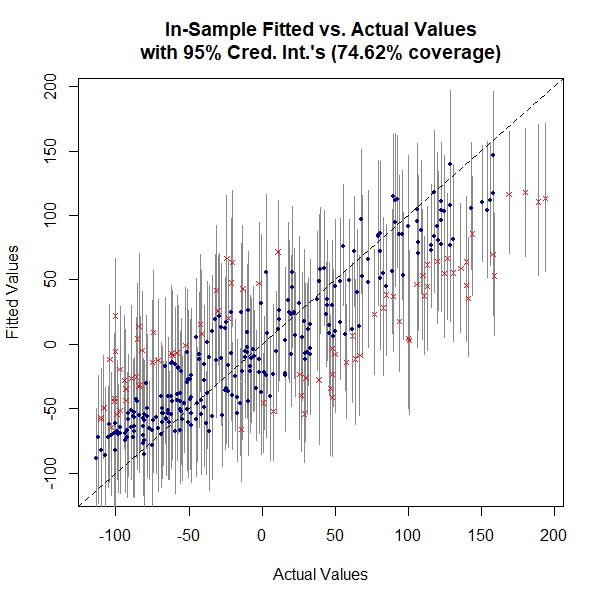
\includegraphics[width=0.6\textwidth]{images/CI.png}
\caption{The plot of in-sample fitted values against actual values show that 74.62\% of the dataset actually have their ground truths lie within the 95\% credible interval .}
\label{CI}
\end{figure}

The plot shows that in overall, most of the predicted values lie around the diagonal of the plots. While the credible interval is set to 95\%, only 74.62\% of the dataset actually have their ground truths lie within the 95\% credible interval of the posterior distribution. This is due to the fact that the credible interval does not take into account of the regularization uncertainty term as discussed in the section \ref{prior}. The author of bartMachine additionally implemented a prediction interval term which takes the regularization uncertainty term into account, giving larger intervals for each dataset. This is performed with the command \textit{plot\_y\_vs\_yhat(bart\_machine, prediction\_intervals = TRUE)} and the resulting plot is shown in Figure \ref{PI}.

\begin{figure}[h!] 
\centering
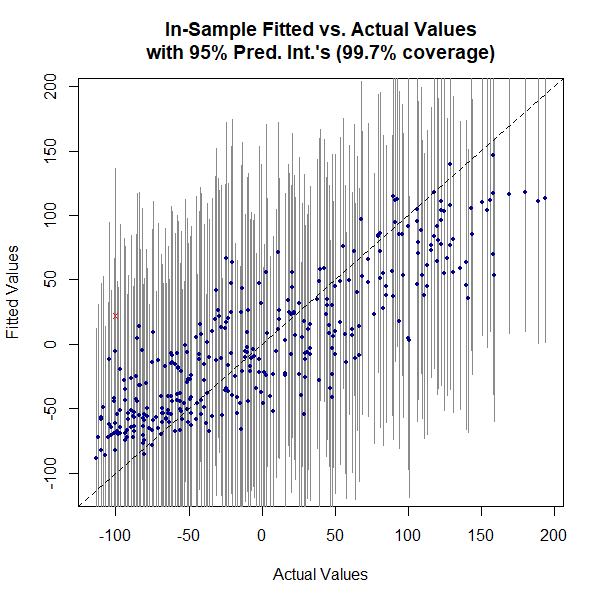
\includegraphics[width=0.6\textwidth]{images/PI.png}
\caption{The plot of in-sample fitted values against actual values show that 99.7\% of the dataset actually have their ground truths lie within the 95\% prediction interval .}
\label{PI}
\end{figure}

From the figure, we can see that the with the regularization error considered, 99.7\% of the dataset actually have their ground truths lie within the 95\% prediction interval of the posterior distribution. Thus, we can see that the model performs reasonably well with the training dataset. Additionally, the 10-fold cross validation RSME of the model is observed to be 56.9, while the 10-fold cross validation pseudo R-squared of the model is observed to be 0.45. These are obtained by the command \textit{k\_fold\_cv(x\_train, y\_train, k\_folds = 10)}. The out-of-sample performance of our BART model is also tested against the test dataset with the command \textit{oos\_perf = bart\_predict\_for\_test\_data(bart\_machine, x\_test, y\_test)}. We obtain an out-of-sample test RMSE value of c. This is about 33\% higher than the in-sample-RMSE values, which also mean that the bartMachine model overfits slightly to the train dataset with the current default hyperparameter values. We will investigate if altering the prior hyperparameters and specifications might result to less overfitted predictions in the hyperparameter optimization section.


The command \textit{rmse\_by\_num\_trees(bart\_machine, num\_replicates = 20)} allows us to plot the RSME of the models against the number of trees used, whereby the average RSME of the 20 replicates of the models are used for the evaluation. The plot is shown in Figure \ref{RMSEtrees}.

\begin{figure}[h!] 
\centering
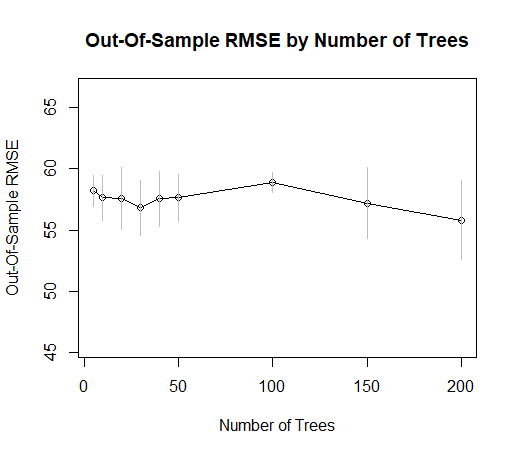
\includegraphics[width=0.6\textwidth]{images/RMSEtrees.png}
\caption{The plot of out-of-sample RMSE by the number of trees for our bartMachine model. We can then deduce which number of trees results to the best out-of-sample RMSE.}
\label{RMSEtrees}
\end{figure}

While the out-of-sample RMSE generally decreases with increasing number of trees, we can observe that the RMSE actually increases after reaching a local minimal value at m = 40 trees, reaching a maximum RMSE value at m = 100 trees and decreasing again up to a minimum value at m = 200 trees. Thus, for our bartMachine model with our current dataset, larger amount of trees do not result to a significantly more generalizable BART model. The overfitting problem is not resolved as well as the out-of-sample RMSE values do not decrease towards the value of our in-sample RMSE value no matter how many trees are used for the modelling. One may prefer to have a smaller amount of trees for similar performance with smaller model sizes and less complexities. The number of trees is one of the hyperparameters that can be tuned to obtain the most optimal performing BART model, which will be discussed in a later section.

\subsubsection{Assumption checking}
The bartMachine provides two tests to check the assumptions that one normally use for regression, namely the test of normality of the residuals ( Shapiro-Wilks p-value test ) and the residual variance test ( Heteroskedasticity test ). This is performed by running the command \textit{check\_bart\_error\_assumptions(bart\_machine)}. The resulting plans are shown in figure \ref{ErrorAss}.

\begin{figure}[h!] 
\centering
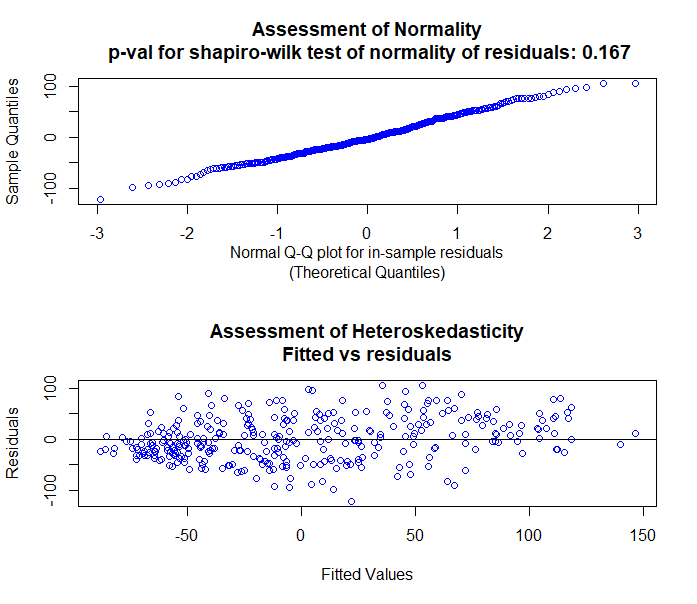
\includegraphics[width=0.7\textwidth]{images/ErrorAss.png}
\caption{The Q-Q plot and heteroskedasticity plot of the residuals. Both plots show that the residuals follow a normal distribution}
\label{ErrorAss}
\end{figure}

From the p-value of 0.167 , the null-hypothesis that the residual follows a normal distribution is not rejeceted, thus we can conclude that the residual indeed follows a normal distribution. This is to be expected as the training sample size n = 331. This is also confirmed visually from the QQ plot, whereby the points roughly lie on the diagonal of the plot. The heteroskedaticity plot also confirms that the residuals are roughly equal across the range of dataset values. Thus we can also observe that the assumptions for our BART model is fulfilled.

\subsubsection{MCMC convergence analysis}
The bartMachine also allows us to monitor the MCMC convergence diagnostics through both the trace of the residual value $\sigma^2$ and the trees parameters across iterations. This is performed by the command \textit{plot\_convergence\_diagnostics(bart\_machine)}. The result of the MCMC convergence diagnostics is shown in Figure \ref{MCMCConv}.

\begin{figure}[h!] 
\centering
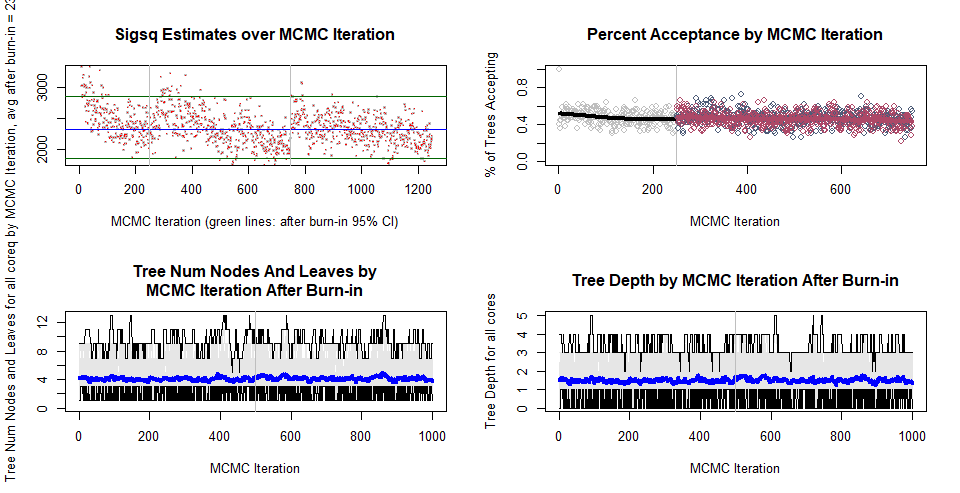
\includegraphics[width=\textwidth]{images/MCMC_convergence.png}
\caption{The MCMC convergence diagnostic plots of (top left) the residual term $\sigma^2$ over iterations, (top right) the Metropolis-Hastings tree acceptance rate over iterations, (bottom left) the number of leaves per trees over iterations, and (bottom right) the depth of trees over iterations.}
\label{MCMCConv}
\end{figure}

There are 4 plots produced by the convergence diagnostic command. The first plot on the top left is the plot of residual term $\sigma^2$ over post burn-in iterations. While the $\sigma^2$ values fluctuated slightly, the fluctuations mostly lie within the 95\% credible interval of the variance of the residual term. Thus, from this plot we can observe that the chain explores the different parts of the sample space of residuals multiple times. The second plot on the top right shows the acceptance rate of the the Metropolis-Hastings part in each Gibbs iteration. The grey part on the left half of the figure indicates the burn-in period, while the right half indicates the post burn-in period. Interestingly, the acceptance rate does not differ significantly during burn-in period and after burn-in period. The third plot in the bottom left is the plot of the trace of the number of nodes per tree over post burn-in iterations. The blue line indicates the average number of nodes and leaves per tree, while the upper bound and lower bound values are indicated with black lines. The number of nodes and leaves does not differ significantly over the post burn-in iterations. Lastly, the plot in the bottom right is the plot of the depth of the trees over post burn-in iterations. Similar to the previous plot, the blue line indicates the average depth of the trees with the upper bound and lower bond values indicated with black lines. Likewise, the depth of the trees do not vary significantly over post burn-in iterations. Since these four plots show the relative stability of the parameters of the model, we can conclude that the chain has indeed converged to the posterior distributions after burn-in given the prior models proposed.

\subsubsection{Hyperparameter optimization}
The bartMachine library also has a built-in hyperparameter optimization functionality, which allows one to easily optimize the hyperparemeters used for the prior modelling via cross-validations. This is done with the command \textit{bart\_machine\_cv <- bartMachineCV(x\_train, y\_train)}, whereby different combinations of the parameters $k, \nu, q,$ and $m$ are applied and the cross-validation errors are evaluated. The winner sets of hyperparameters which result to the lowest cross-validation error values are then applied to build a new optimized bartMachine model. For our current BART model, the winning hyperparameter combination is  $k = 2, \nu = 0.9, q = 3,$ and $m = 50$, which is thus the same hyperparameter combination used in our default bartMachine model. For our dataset, it is thus not necessary to optimize the hyperparameters further. The in-sample, test and cross validation RSME and pseudo R-square values of the optimized model are summarized in the following table.

\begin{table}[h!]
\centering
\caption{Table of RMSE and Pseudo $R^2$ values of the bartMachine BART model.}
\begin{tabular}{|c|c|c|c|}
\hline & In-sample & 10-fold CV & Test \\
\hline RMSE & 41.6 & 56.9 & 56.1 \\
\hline Pseudo $R^2$ & 0.71 & 0.45 & 0.50 \\ \hline
\end{tabular}
\label{RMSEBART}
\end{table}

\subsubsection{Variable Importance and Partial Dependence}
Since there are a total of 64 covariates in the dataset, we would like to investigate which variables are considered more important for the prediction of our BART model. This can be performed by the command \textit{investigate\_var\_importance(bart\_machine, num\_replicates\_for\_avg = 20)}. The plot is shown in Figure \ref{VarImp}.

\begin{figure}[h!] 
\centering
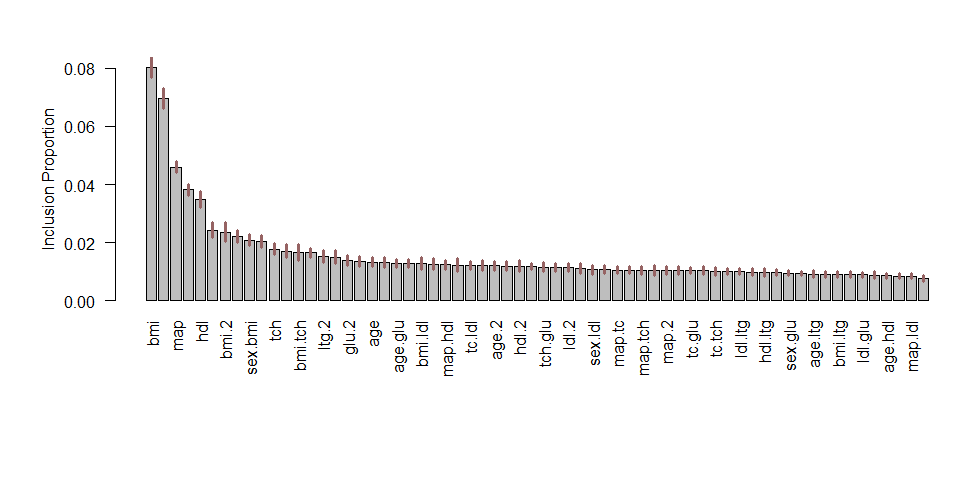
\includegraphics[width=\textwidth]{images/VarImp.png}
\caption{Variable importance plot of the bartMachine model.}
\label{VarImp}
\end{figure}

According to the variable importance plot, the covariates BMI and map ( mean arterial blood pressure ) are the most significant covariates for our bartMachine model. The variable importance plot also shows that out of the 64 covariates ,only the five most important covariates are of significantly higher importances. We may want to investigate the partial dependence plots of the covariates in order to investiage the effect of each covariates to the BART model output in more detail. This can also be done with the bartMachine library through the command \textit{pd\_plot(bart\_machine\_cv, j = "bmi")} for example. The partial dependence plots of the two covariates with the highest importance values are shown in the following figures.

\begin{figure}[h!] 
\centering
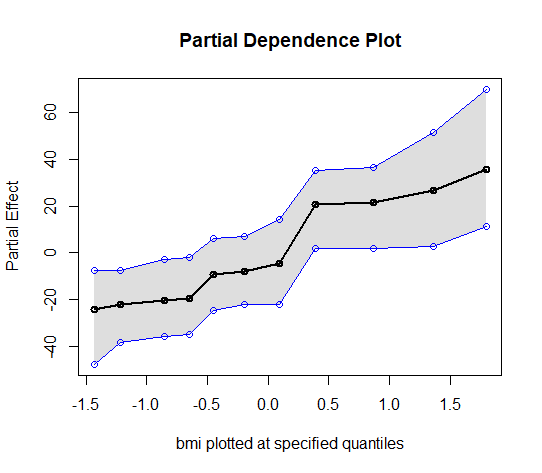
\includegraphics[width=0.7\textwidth]{images/PD_BMI.png}
\caption{Partial dependence plot of the BMI covariate.}
\label{PDBMI}
\end{figure}

\begin{figure}[h!] 
\centering
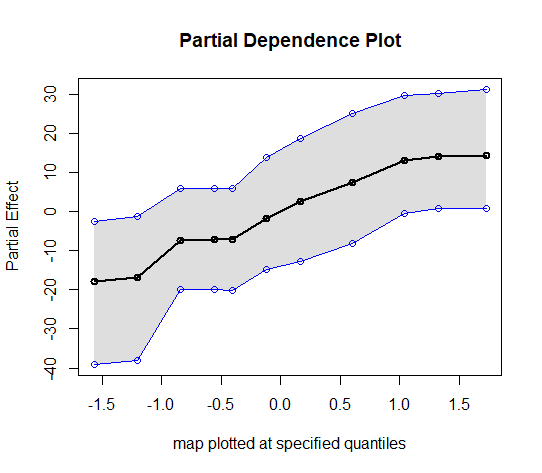
\includegraphics[width=0.7\textwidth]{images/PD_map.png}
\caption{Partial dependence plot of the map covariate.}
\label{PDmap}
\end{figure}

From both plots, we can observe that changing the values of BMI and map covariate change the output values significantly. There seems to be a steeper gradient increase for BMI covariate values between the quantile 0 and 0.5 and the same can be observed for the map covariate values between quantile -1.25 to -0.75. Thus we can observe that the relationship between the output and the covariate values are not strictly linear. It would also be interesting to investigate the partial dependence plots of the many other covariates, however this is left out for future  studies and analysis. The BART model is thus able to model non-linear relationships significantly well. 

\subsection{Second experiment results : Performance Comparison}
\subsubsection{"BART" library}
As a comparison, a BART model is also constructed from the "BART" with the default settings. While most of the prior modelling and default parameters are similar, there are differences to some of the default hyperparameters and some model assumptions as highlighted by Kapelner and Bleich in their bartMachine publication \cite{11}. The BART model implementation from the "BART" library is closer to the original BART publication by Chipman e.t. al. The main differences in the hyperparmeter setting are that in the "BART" library, the default number of tree is taken to be m = 200, burn-iteration is taken to be 100 iterations, and the post burn-in iteration is taken to be 1000 iterations. The modelling and training takes 3 seconds in our local machine. While for bartMachine , it takes 2 seconds in our local machine. The obtained test-set RMSE value is 55.5 which is about 10\% better than the test-set RMSE value from the bartMachine implementation. While there are slight improvements in the RMSE value, if the different implementations and modelling assumptions significantly result to a significant difference in performance. An in detail significance testing and performance study can be done to investigate this into more detail. This is not included within the scope of our current study.

\subsubsection{Classic CART}
Regression trees are generated through the rpart package in R. We fit the model on the training data by setting method="anova" as we are working in a regression setting. The regression tree is shown in Figure \ref{CART1}. 

\begin{figure}[h!] 
\centering
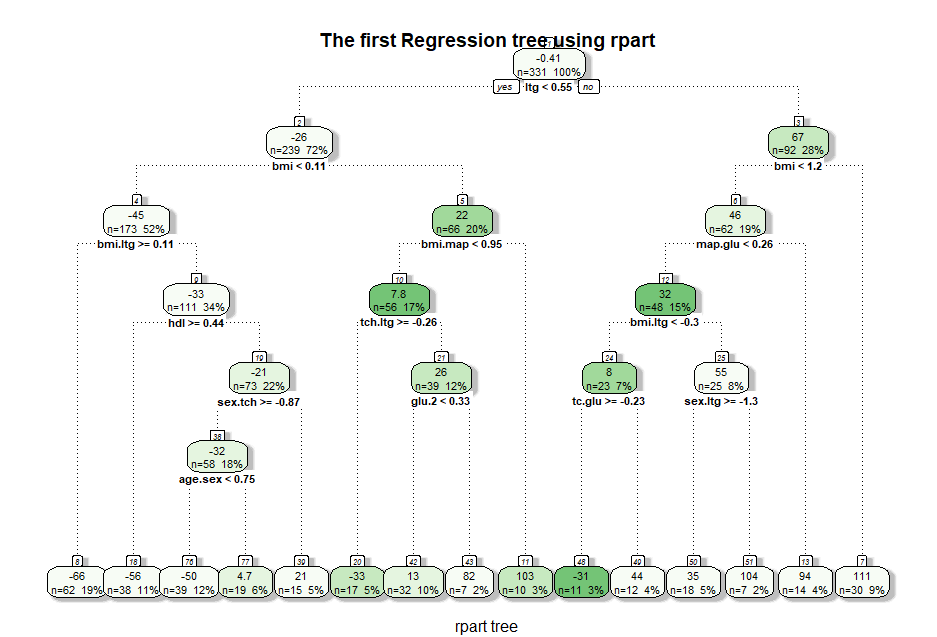
\includegraphics[width=0.7\textwidth]{images/image107.png}
\caption{The first regression tree using rpart.}
\label{CART1}
\end{figure}

To compare the error for each cp value, cross-validation is performed such that the error related with a given cp value is computed on the hold-out validation data. In figure \ref{CARTcv} such a plot is shown, where the y-axis is the cross-validation error, the lower x-axis is the cp value and the upper x-axis is the number of terminal nodes. From the plot we see that the best value of cp, resulting in the lowest cross-validation error, is for cp=0.0426. This value of cp is used in the next section to perform pruning of the tree. 

\begin{figure}[h!] 
\centering
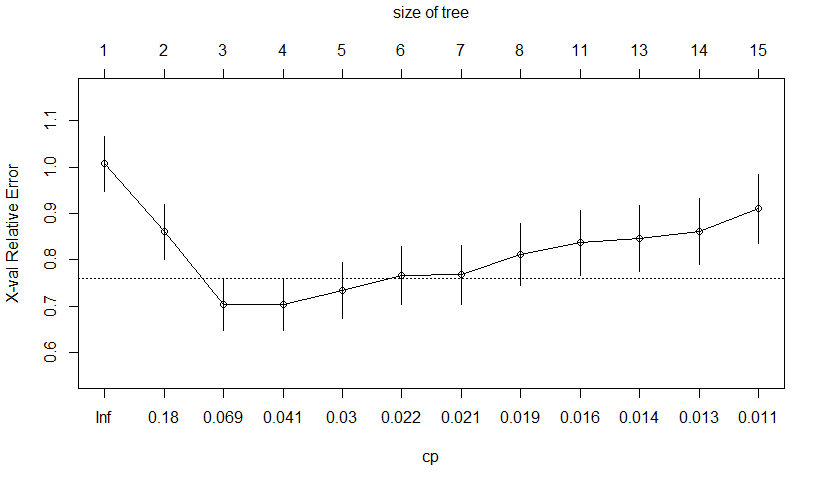
\includegraphics[width=0.7\textwidth]{images/image111.png}
\caption{Plot of the cross validation results for the tree across different cp values.}
\label{CARTcv}
\end{figure}

The tree is pruned to avoid overfitting, by minimizing the cross-validation error - xerror. This is performed through automatic selection of the complexity parameters associated with the smallest cross-validation error. The pruned tree is displayed in figure \ref{CARTpruned}. In addition, the 10-fold cross validation repeated 10 times is used to help us find the best combinations of algorithm parameters for our classification problem by tuning the model parameters. In order to achieve such tuning, the CARET package of R, which stands for Classification and Regression Training, is being used. The 10-fold cross validation is repeated 10 times by specifying the method parameter and the repeats parameter of the trainControl function to "repeatedcv" and 10 respectively. In this way, each subset is used at least once for training the classifier, and the average performance on all the 10 folds is outputted. The model is tuned through the complexity parameter (cp). Moreover, the tuneLength parameter , which makes the model try different default values for the main parameter cp, is set to 100. This means that the total number of combinations evaluated is 100. Figure \ref{CARTtune} displays how the change in cp value affects the RMSE value. RMSE was used to select the optimal model using the smallest value. As it can be seen in the plot, the final value used for the model was cp = 0.033 with RMSE=62.8 and $R^2$=0.36 in the training set, and with RMSE = 63.9 and $R^2$= 0.33 in the test set. An R squared of 0.33 tells us that our model explains only 33\% of the variation in the data.

\begin{figure}[h!] 
\centering
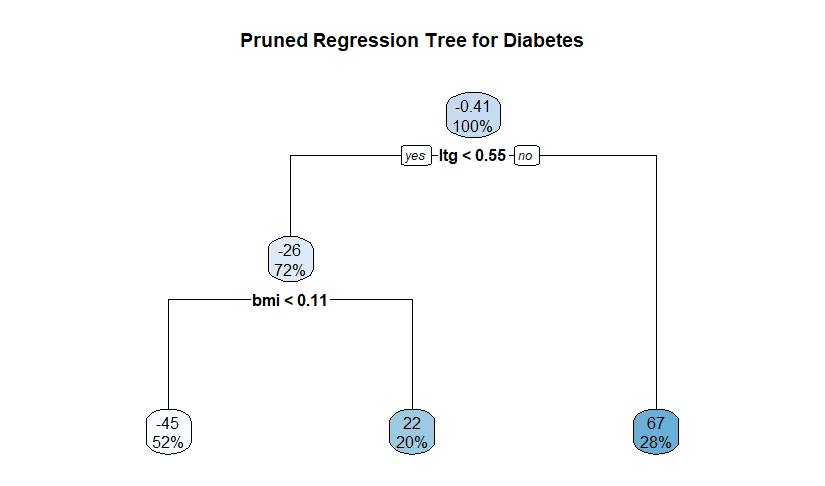
\includegraphics[width=0.7\textwidth]{images/image124.png}
\caption{The pruned regression tree.}
\label{CARTpruned}
\end{figure}

\begin{figure}[h!] 
\centering
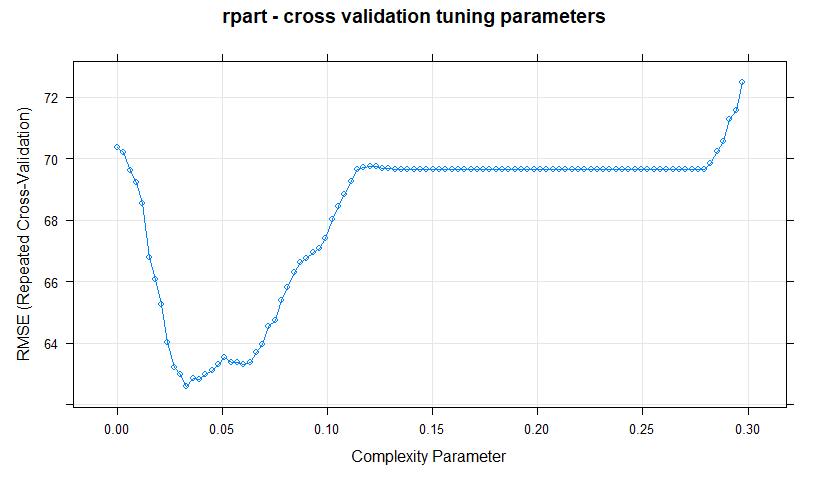
\includegraphics[width=0.7\textwidth]{images/image127.png}
\caption{Plot of cross validation RSME against tuning complexity parameters.}
\label{CARTtune}
\end{figure}

In addition to tuning the cp value, we perform further tuning of minsplit and maxdepth. minsplit represents the minimum number of data points required to split a node before making it terminal, while maxdepth represents the maximum number of internal nodes.  To do so, grid search is used to automatically search across a range of differently tuned models to recognise the most optimal parameter setting with the highest performance. The search range of minsplit is set from 5-20 and the search range of maxdepth is set from 1-15, which results in 240 different combinations. It results that the lowest error is achieved with minsplit = 13, maxdepth = 3 and cp = 0.023. However, comparing such a model with the previous model, where we did cross-validation and cp tuning, we observe that the both models perform quite the same in terms of RMSE and R-squared (see Table \ref{CARTresults}). However, we see a much better performance of the model after performing 10-fold cross-validation and identifying the most optimal cp value, compared to the initial tree with default parameter setting or the pruned tree. The final regression tree after performing parameter tuning is shown in Figure \ref{CARTfinal}.

\begin{table}
\centering \caption{Regression tree models comparison.} \label{CARTresults}
\begin{tabular}{|c|c|c|c|c|}
\hline & Initial tree with default parameters & Pruned tree & 10-fold cross validation tree & Tuned tree \\
\hline RMSE on test set & $65.78$ & $68.02$ & $63.9$ & $63.9$ \\
\hline R Squared on test set & $0.33$ & $0.25$ & $0.33$ & $0.33$ \\
\hline
\end{tabular}
\end{table}


\begin{figure}[h!] 
\centering
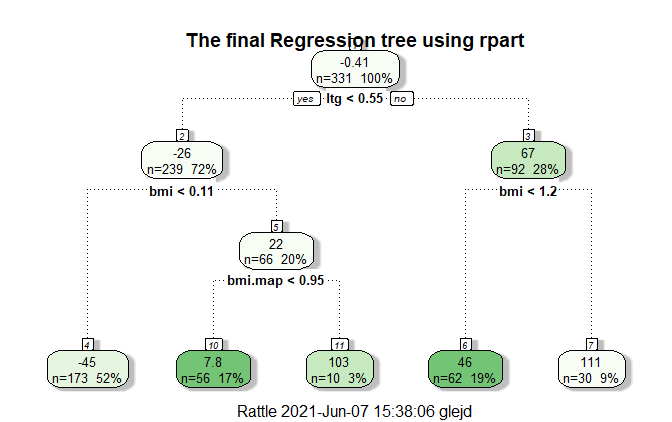
\includegraphics[width=0.7\textwidth]{images/image110.png}
\caption{Final regression tree after parameter tuning.}
\label{CARTfinal}
\end{figure}


Lastly, the barplot of the variables that have the most largest weight in the prediction are plotted in figure \ref{CARTimp}. It is clear that ltg, bmi, bmi.ltg, tc, and bmi.2 are the top 5 most important variables in our regression model. 

\begin{figure}[h!] 
\centering
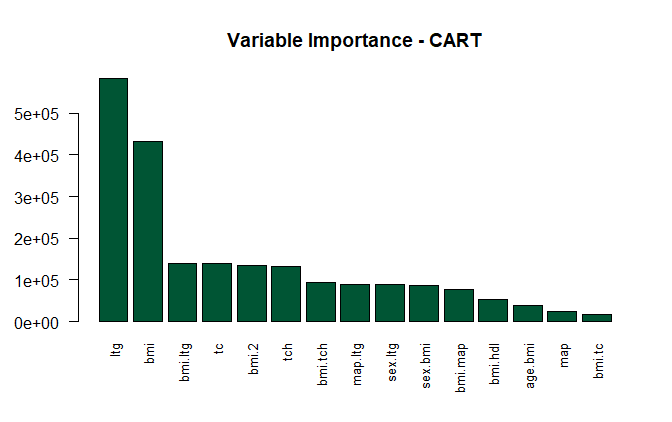
\includegraphics[width=0.7\textwidth]{images/image112.png}
\caption{Final regression tree after parameter tuning.}
\label{CARTimp}
\end{figure}

\subsubsection{Random Forest}
As mentioned before, in RF each tree is allowed to grow to a bootstrap resampled data set, and an advantage of it is the fact the RF has an out-of-bag (OOB) sample which gives a good and efficient approximation of the test error. The plot in figure \label{RFOOB} shows the OOB error versus the validation error for the random forest. As expected, there are some differences between them. The out-of-bag error seems to be constantly higher than the test error. 

\begin{figure}[h!] 
\centering
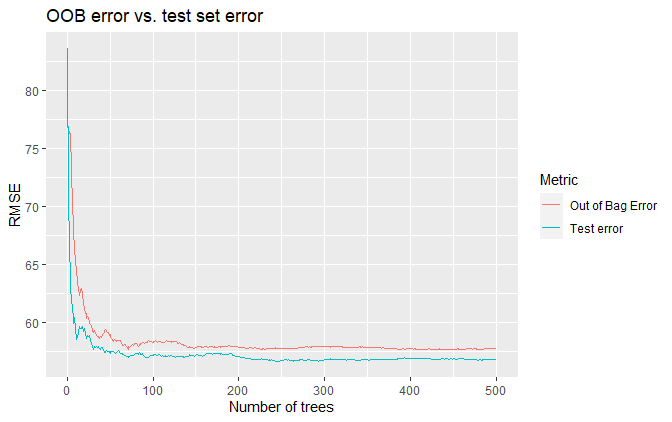
\includegraphics[width=0.7\textwidth]{images/image125.png}
\caption{Random forest out-of-bag error versus validation error.}
\label{RFOOB}
\end{figure}

In figure \ref{RFtrees}, the plot of the random forest model with default parameter setting is shown. The plot illustrates the error rate as we increase the number of trees in the model. The error rate seems to stabilize with 100 trees, but it still continues to decrease even with a bigger number of trees at a much slower rate. According to this plot, the number of trees with the lowest MSE of 57.7 is 479 trees. However, to define the best parameter setting, tuning was performed in the model, which is described in more detail in the next section. 

\begin{figure}[h!] 
\centering
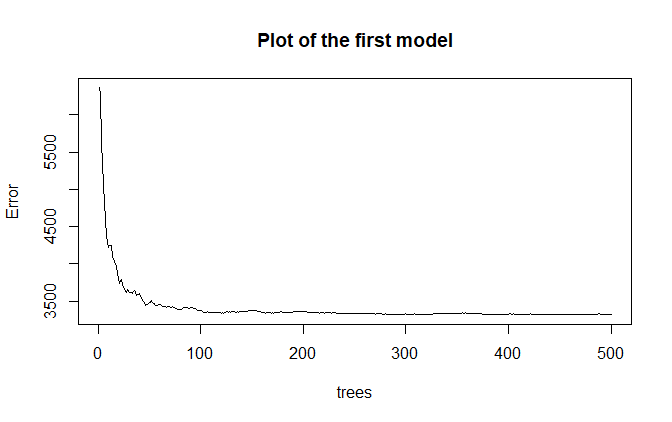
\includegraphics[width=0.7\textwidth]{images/image118.png}
\caption{Plot of the error of the first RF model with default parameter setting against number of trees.}
\label{RFtrees}
\end{figure}

RF is mainly controlled by four parameters: mtry stands for the number of variables randomly sampled as candidates at each split, maxnodes stands for the depth of the tree, nodesize stands for the maximal number of observations in each cell, and ntree stands for the number of trees allowed to grow \cite{26}. Hence, 10-fold cross validation is used to identify the optimal parameter setting. To tune the model, a grid of 1-50 is defined by setting the search parameter of TrainControl function to "grid", where each point in the grid represents a specific combination of parameters. In order to select the most optimal model, RMSE was used for selection using the smallest value, aiming for the lowest error, and so the best performance. First, a search for the best mtry is conducted. Figure \ref{RFRMSE} shows how the RMSE value changes with respect to the number  of variables used in the model, mtry score. As a result, the lowest RMSE score is obtained with a value of mtry equals to 10. As it can be clearly seen from the plot, there is a great drop in the cross-validation error from 0-10 randomly selected predictors, and after 10 there is a slow increase in the error. 

\begin{figure}[h!] 
\centering
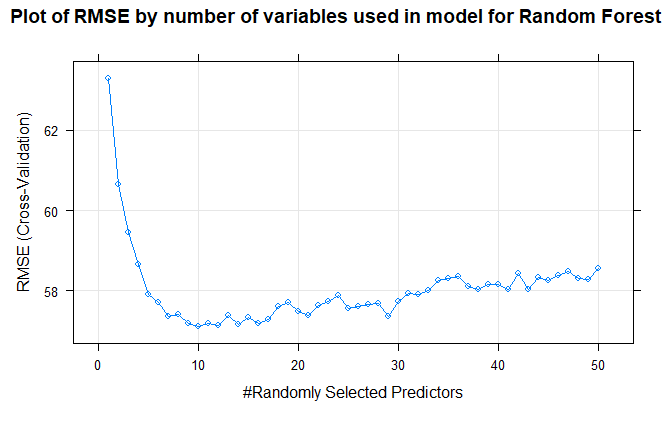
\includegraphics[width=0.7\textwidth]{images/image121.png}
\caption{Plot of RMSE by number of variables used in the model for RF.}
\label{RFRMSE}
\end{figure}

Next, we search for the best maxnodes parameter value. This is done in iterations, with the range being enlarged by ten in each iteration to attain the lowest RMSE. The lowest RMSE score of approximately 46.8 and the better R-squared value of 0.232 is obtained with a value of maxnode equals to 11.  The final parameter tuning is done to find the best ntrees score. This is performed by taking a vector [10, 50, 100, 250, 300, 350, 400, 450, 500, 550, 600, 800, 1000]. As a result, ntree equal to 50 seems to be the most optimal choice, both in terms of RMSE and R-squared values. Finally, the RF model is trained with the following parameter setting: maxnodes = 11, mtry = 10, ntree = 50. As a result, the RMSE on the test set is 56.8, while the R-squared = 0.47. Moreover, as it can be seen from the table below, after tuning we did not receive better results, as expected otherwise. 

\begin{table}
\centering \label{RFtuned} \caption{Random forest model comparison before and after parameter tuning.}
\begin{tabular}{|l|l|l|}
\hline & Initial RF with default parameters & RF with tuned parameters \\
\hline RMSE on test set & $56.8$ & $56.8$ \\
\hline R Squared on test set & $0.465$ & $0.469$ \\
\hline
\end{tabular}
\end{table}

The 5 most important features for the random forest based on node purity are ltg, bmi, map, bmi.ltg, bmi.2 as shown in Figure \ref{RFImp}, while based on MSE value ltg, bmi, map, tch, mpa.glu. Comparing these with the results of the CART, we see that the features with the highest weight in prediction are almost the same. 

\begin{figure}[h!] 
\centering
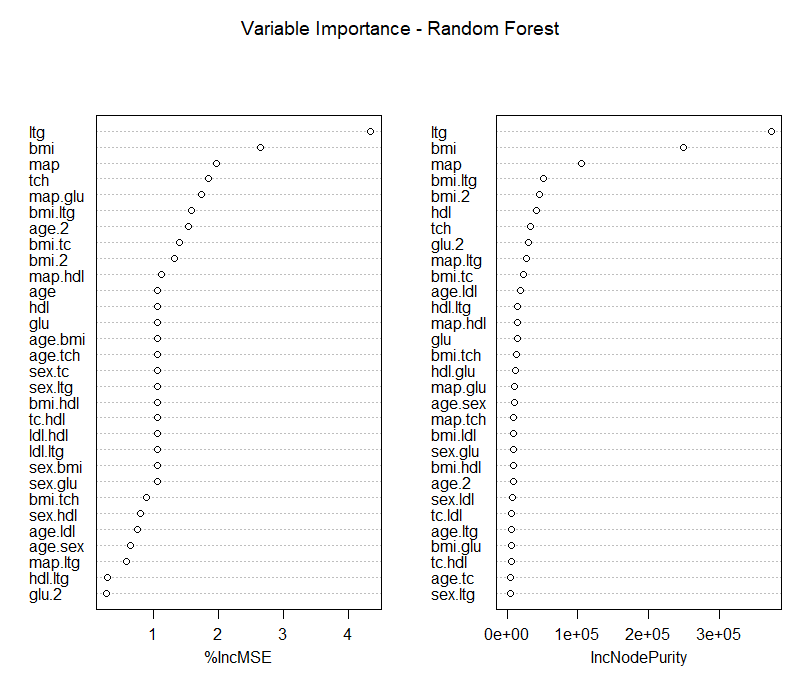
\includegraphics[width=0.7\textwidth]{images/image115.png}
\caption{Variable importance for random forest.}
\label{RFImp}
\end{figure}

\subsubsection{Results Discussion}
The performance of the different models on diabetes dataset are summarized in the Table \ref{result_diabetes}. Note that the values for the regression tree is taken from the best optimized regression tree as obtained previously. 

\begin{table} 
\centering \caption{Performance metrics of the different models on diabetes dataset.}
\begin{tabular}{|c|c|c|c|c|} 
\hline &  Regression Tree & Random Forest & bartMachine & BART \\
\hline RSME on test set & 63.9 & 56.8 & 56.1  & 55.5 \\
\hline $R^2$ on test set & 0.33 & 0.47 & 0.50  & 0.53\\
\hline
\end{tabular}
\label{result_diabetes}
\end{table}

In general, our BART models perform significantly better than the most optimized version of the regression tree model. Meanwhile, the performance improvement is marginal compared to the random forest model. Interestingly, the BART model implemented by the BART library performs marginally better than the bartMachine implementation, which may be due to the different prior hyperparameter values and prior modelling assumptions taken by the publisher of both R libraries. In conclusion, BART shows to be a very promising alternative to other very commonly used regression machine learning methods.

\subsection{Third experiment results : Friedman Data}
The dataset specification can be found in the \ref{dataset} section. The results from the third experiment are summarized in Table \ref{result_table}.

\begin{table} 
\centering \caption{Performance metrics of the different models on Friedman dataset.}
\begin{tabular}{|c|c|c|c|} 
\hline & Regression Tree & Random Forest & BART \\
\hline RSME on test set & 2.93 & 2.51 & 1.61 \\
\hline $R^2$ on test set & 0.62 & 0.78 & 0.88 \\
\hline
\end{tabular}
\label{result_table}
\end{table}

From the results we can see that BART significantly outperform classic regression tree and random forest models for the synthetic Friedman dataset. BART is able to decide better on the 5 important covariates out of the 100 covariates and perform more accurate predictions in a highly non-linear dataset. In conclusion, this test further shows how BART is a powerful a machine learning model that is able to capture non-linear dependencies in data with high degree of non-linearity. 

\subsection{Discussion of results from other studies}
Scarpone et al. (2020) \cite{16} analyze only the first wave of COVID-19 data in Germany using the BART model to identify important socioeconomic and infrastructural covariates with the number of incidents. They conclude that the implemented measure of social distancing and border restrictions are important in reducing the spread of COVID-19 infections, as the incidence rates are dependent on the geographical location, transportation infrastructure and the labor market structure of the county. Moreover, in the paper, it is concluded that BART is a very powerful machine learning tool for modelling non-linear data in high dimensional space, and that the model can be entirely explained from only a subset of the variables \cite{16}.  

Kapelner and Bleich (2016) \cite{14} introduce the bartMachine package in R, which implements the Bayesian Additive Regression trees.  In order to show the effectiveness and efficiency of such a package, they perform a BART analysis on the automobile dataset from UCI Machine Learning Repository to predict the automobile's price from 25 features. Observing the out-of-sample versus in-sample results, they conclude that the model is slightly overfitting. Trying to build a better bartMachine model, a grid search over a set of hyperparameter combinations is performed with the help of barMachineCV function. This returns the best mode with better in-sample performance compared to the default model mentioned above. Furthermore, the MCMC convergence diagnostics is performed. As in many machine learning research, it is natural to ask which variables are the most important ones in prediction. Kapelner and Bleich (2016) perform such analysis \cite{14}. Lastly, they investigate the partial dependence aiming to analyse how $x_j$ affects the response on average. We would like to acknowledge that most of our work in this report paper was based on this publication by Kapelner and Bleich (2016) \cite{14}. 

\section{Limitations and Outlook}
-
-Performance comparison 
-Playing around with the priors, test with other sampling methods
-
\section{Conclusion}
This report paper is focused on analyzing the power of the Bayesian additive regression trees model through a real world application using data from 442 patients diagnosed with diabetes. The dataset contains 10 original feature vectors including information such as age, sex, BMI, BP and the serum measurements, aiming to predic the disease progression one year after the baseline. To show the effectiveness of the BART model, we compare such a model with classical CART and Random Forests. The results show that the default BART model provides more accurate results even compared to already optimized classical CART and Random Forest models. This is confirmed when we assess the comparison in a controlled setting with synthetic Friedman data, whereby we observe that the BART models show a much better performance against high dimensional, non-linear data. We also provided insights into previous studies where we based our experiments on. Lastly, a short insight into current limtations and outlook was provided.

\clearpage
\bibliographystyle{abbrv}
\bibliography{citations}

\clearpage
\section{Appendix}

\begin{figure}[h!] 
\centering
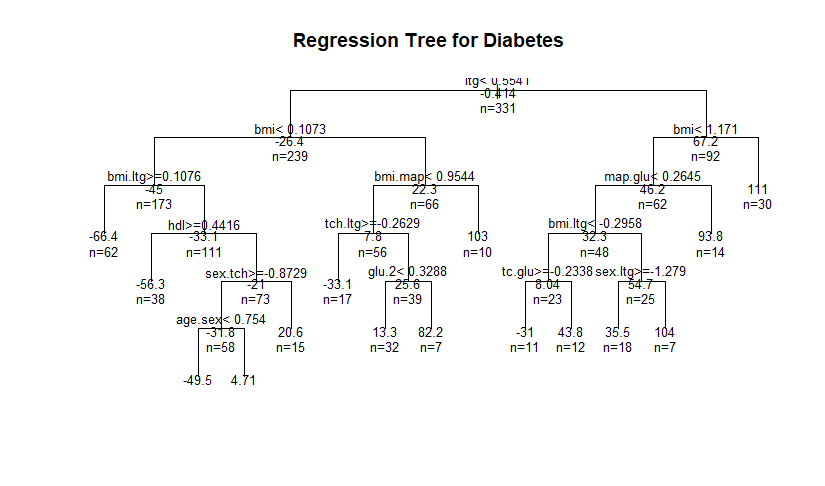
\includegraphics[width=0.7\textwidth]{images/image119.png}
\end{figure}

\begin{figure}[h!] 
\centering
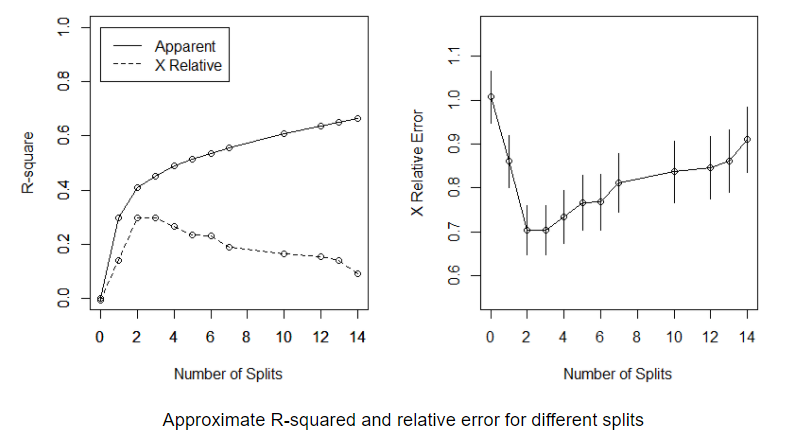
\includegraphics[width=0.7\textwidth]{images/image126.png}
\end{figure}

\begin{figure}[h!] 
\centering
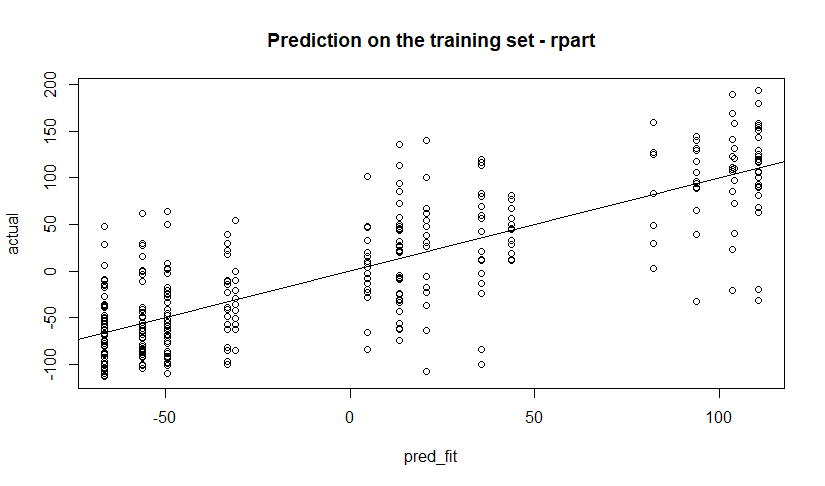
\includegraphics[width=0.7\textwidth]{images/image108.png}
\end{figure}


\begin{figure}[h!] 
\centering
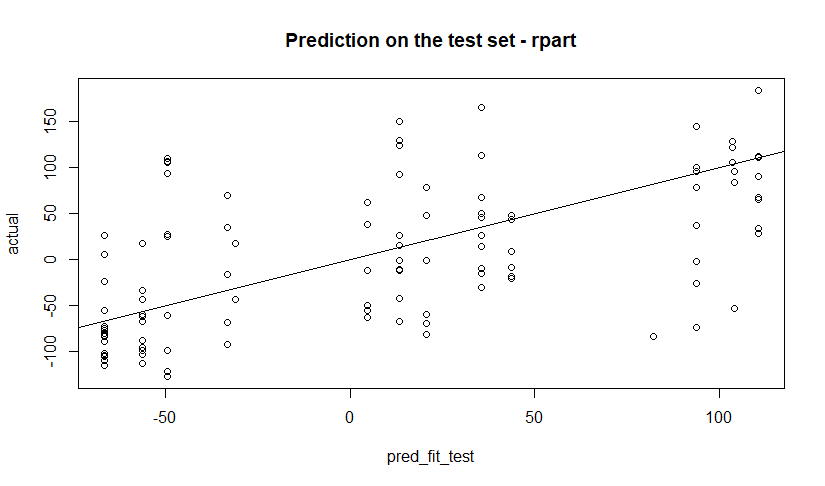
\includegraphics[width=0.7\textwidth]{images/image117.png}
\end{figure}
\end{document}

